\appendix
%%% Оформление заголовков приложений ближе к ГОСТ:
\setlength{\midchapskip}{20pt}
\renewcommand*{\afterchapternum}{\par\nobreak\vskip \midchapskip}
\renewcommand\thechapter{\Asbuk{chapter}} % Чтобы приложения русскими буквами нумеровались
   % Предварительные настройки для правильного подключения Приложений
\chapter{Реализация алгоритма RAP-MUSIC на языке Python}\label{appendix:rap_music_code}

\begin{ListingEnv}[!h]
    \begin{lstlisting}[language=Python,label={rap_music_listing},caption={Алгоритм RAP-MUSIC}]
def RAP_MUSIC(X, G, threshold):
    """
    Параметры
    ---------
    X : матрица измерений
    G : матрица прямой модели для свободной ориентации
    threshold : порог корреляции подпространств

    Возвращает
    ----------
    active_dipole_indices : индексы найденных диполей

    """
    # инициализируем пустой список индексов активных диполей
    active_dipole_indices = []

    while True:
        # ищем корреляции подпространств для каждого источника
        C = MUSIC_scan(X, G)
        if max(C) < threshold:
            break
        k = argmax(C)
        active_dipole_indices.append(k) 
        # проецируем от диполей k-го источника
        X, G = project_away_from_k(X, G, k) 

    return active_dipole_indices
    \end{lstlisting}
\end{ListingEnv}

\chapter{Распределение индуцированной активности по коре в реальных данных}\label{appendix:real_data_power}

Чтобы подтвердить наши выводы и убедиться, что полученные сети не
полностью совпадают с областями коры с доминирующей активностью мы
представили здесь распределение индуцированной активности по коре для целевых частотных диапазонов,
см. рис.~\ref{fig:theta_alpha_pwr},~\ref{fig:beta_pwr},~\ref{fig:gamma_pwr}.
Эти распределения были получены при помощи пакатеа MNE-python в соответствии со следующей процедурой.

Во-первых, чтобы компенсировать разницу в продолжительности эпох из-за
вариабельности времени отклика, мы обрезали каждое испытание в [-0.5, 1.024] секундном
интервале, который соответствовал временному диапазону самой короткой эпохи.
Чтобы смягчить граничные эффекты фильтрации, мы
обратили во времени каждую эпоху и ``приклеили'' ее слев и справа к исходной.
Эти эпохи тройной длины были затем отфильтрованы
в пяти целевых частотных диапазонах КИХ-фильтром с нулевой фазой и переобрезаны
до временного интервала [0,1] секунд, где 0 соответствует моменту предъявления стимула в
исходной неинвертированной эпохе. Далее для пространства источников с 8194
узлами мы вычислили обратный оператор MNE со свободной ориентацией
(коэффициент свободной ориентации = 0,2) и взвешиванием по глубине (коэффициент = 0,6)
и применили его к отдельным испытаниям. Наконец, мы возвели значения для эпох на уровне источников в квадрат и усреднили по времени и по эпохам.
Полученные значения мы нанесли на графики.

\begin{figure}
      \begin{subfigure}[b]{0.5\textwidth}
        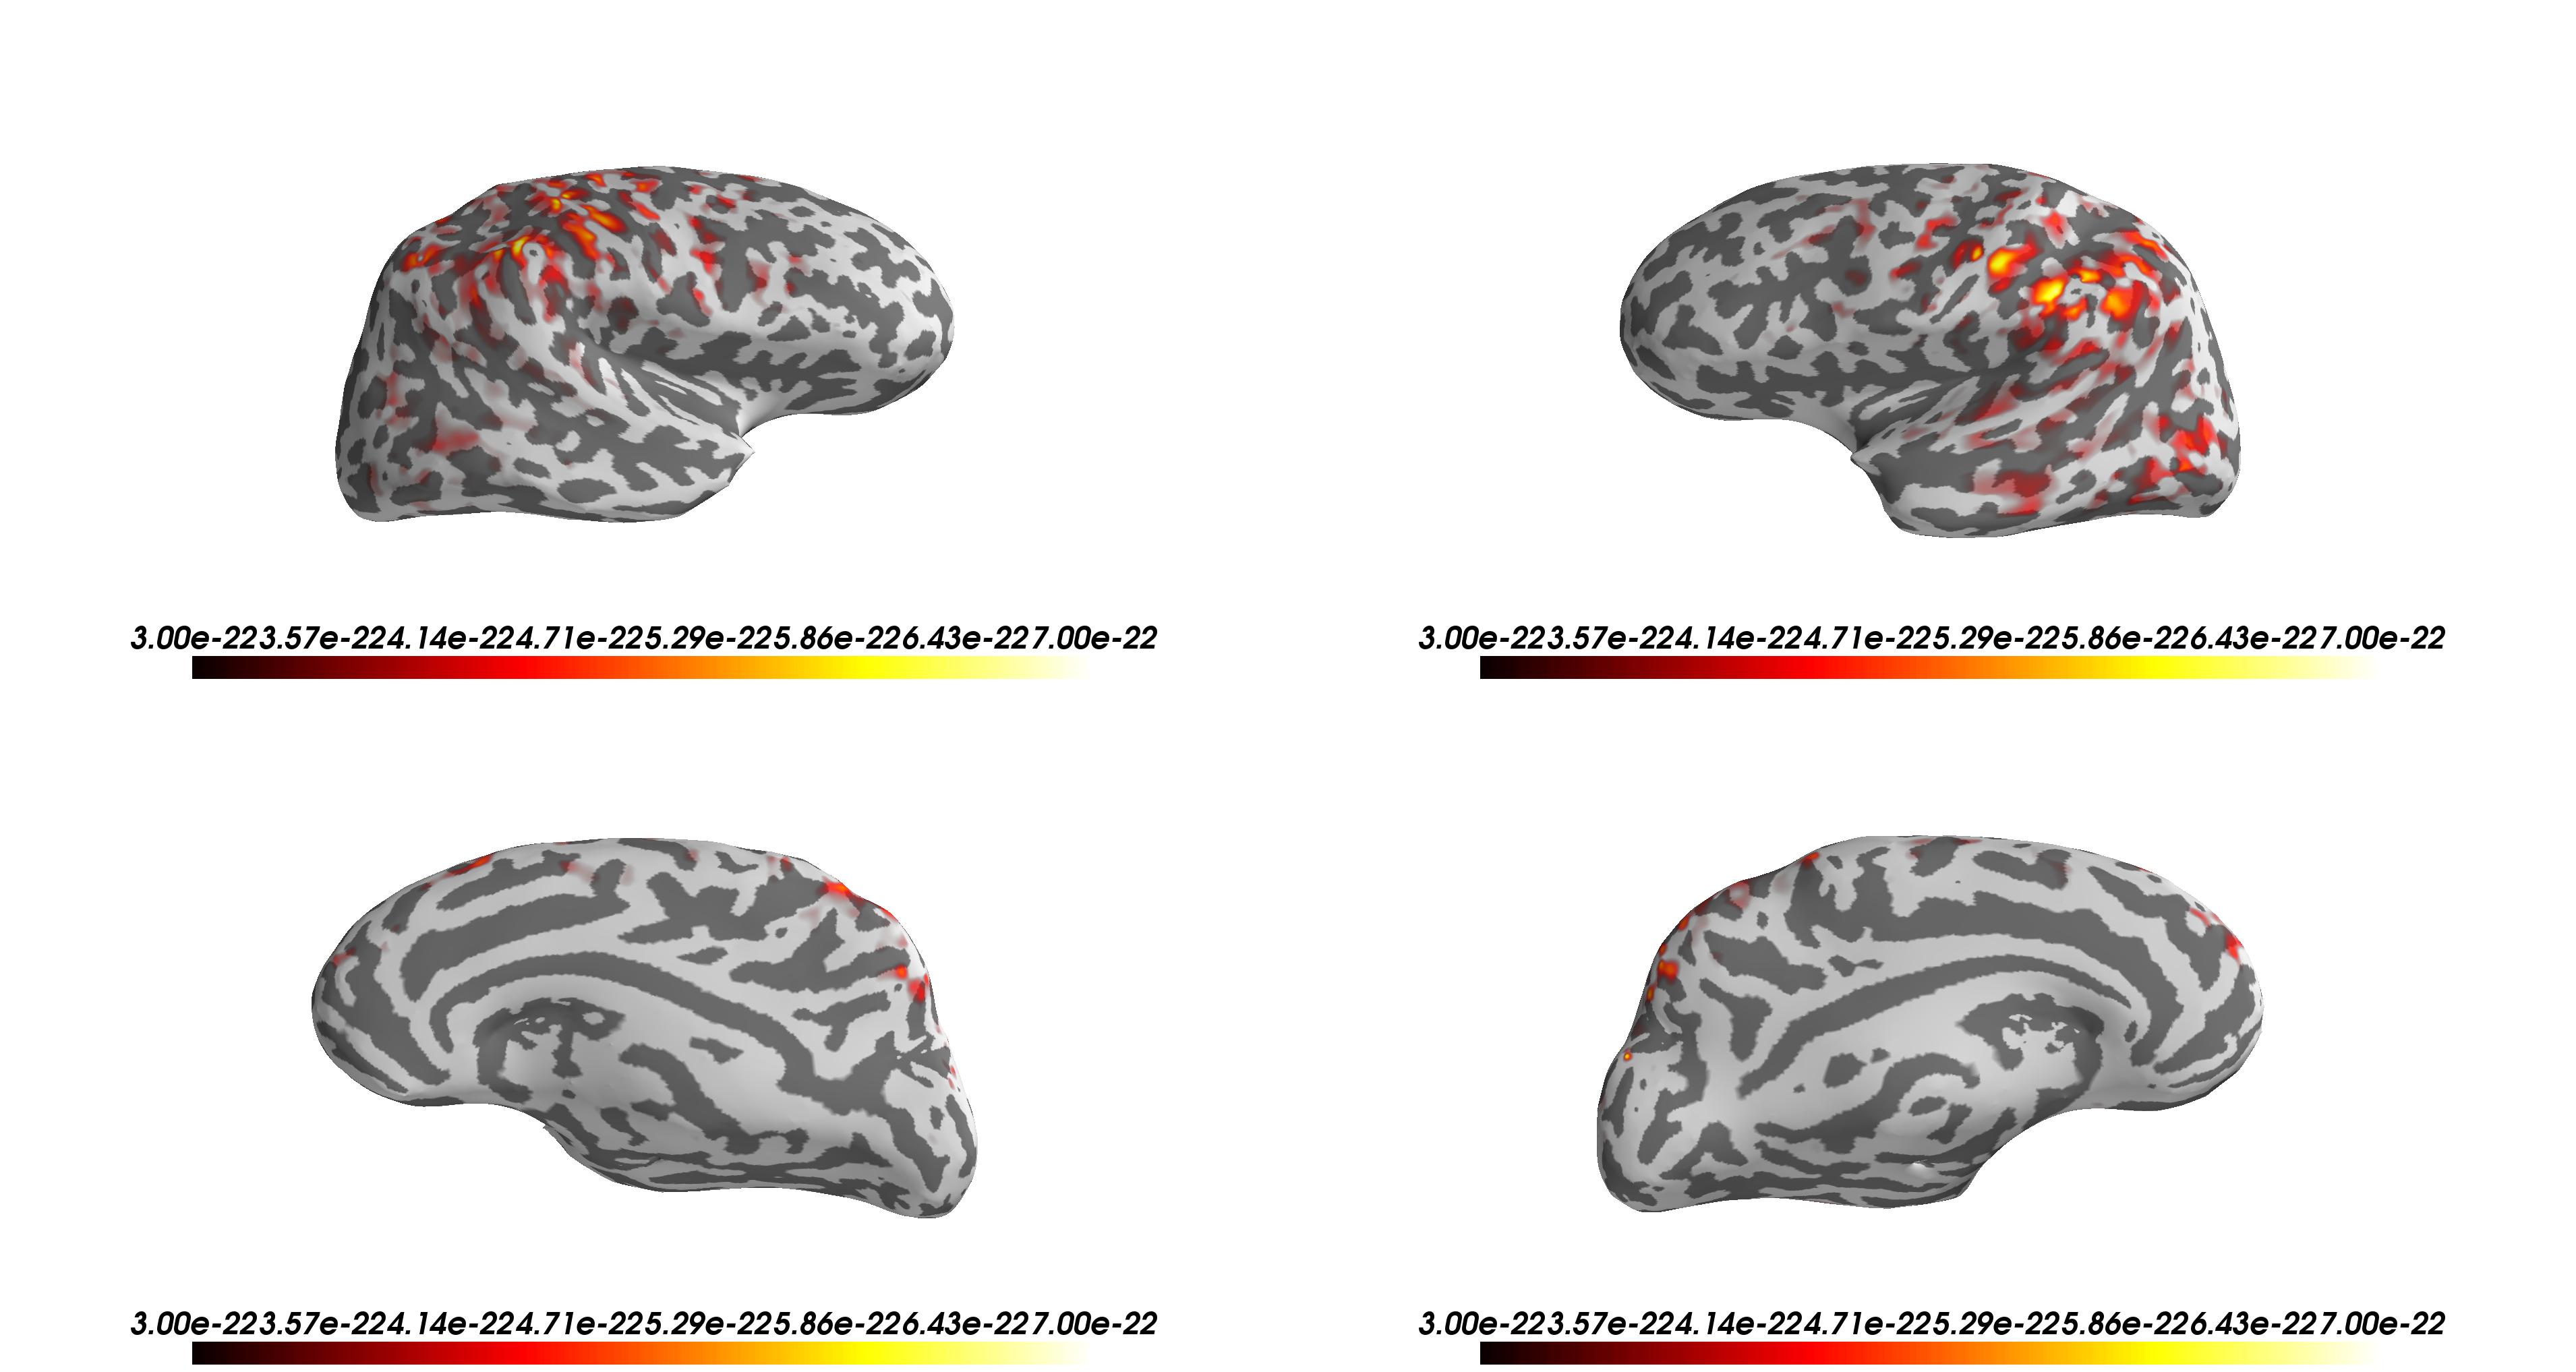
\includegraphics[width=\textwidth]{../images/psiicos_paper/Figure16a_hr.jpg}
        \caption{Тета-диапазон}\label{fig:theta_pwr}
      \end{subfigure}
      % \vspace{1cm}
      \begin{subfigure}[b]{0.5\textwidth}
        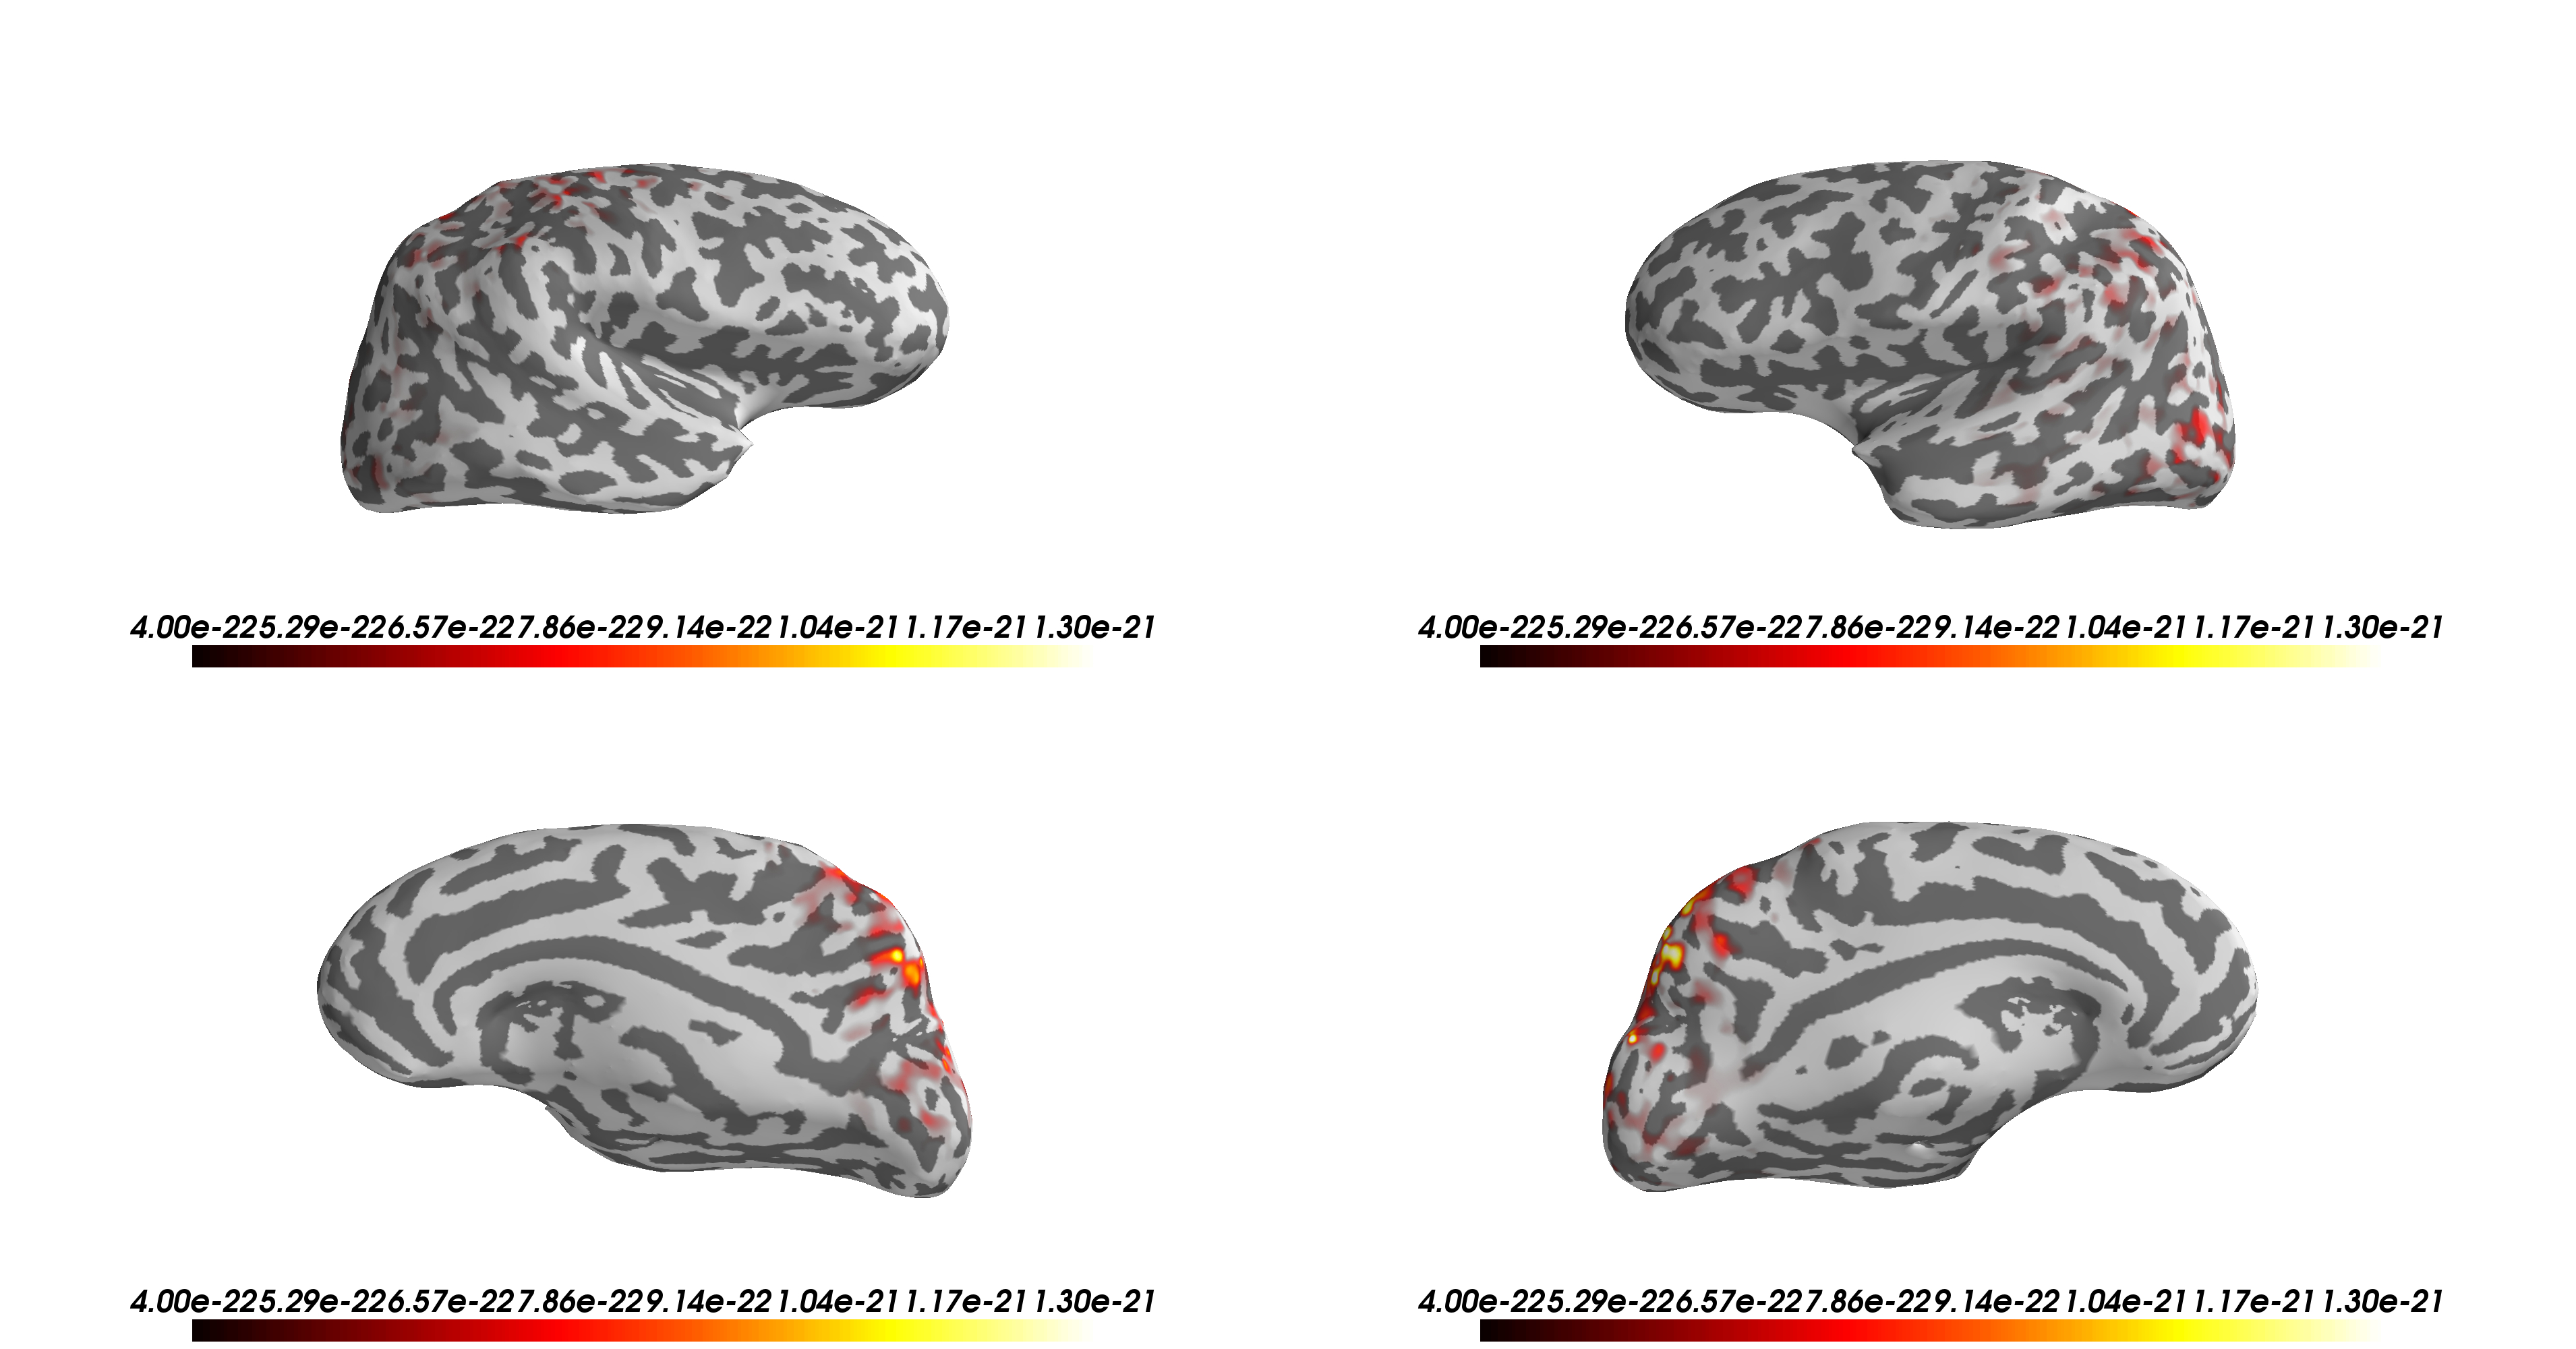
\includegraphics[width=0.99\textwidth]{../images/psiicos_paper/Figure16b_hr.jpg}
        \caption{Альфа-диапазон}\label{fig:alpha_pwr}
      \end{subfigure}
      \caption{Распределение индуцированной активности в тета (3--6 Гц) и альфа (8--12 Гц) диапазонах}\label{fig:theta_alpha_pwr}
\end{figure} %figure 16

\begin{figure}
    \begin{subfigure}[b]{1\textwidth}
    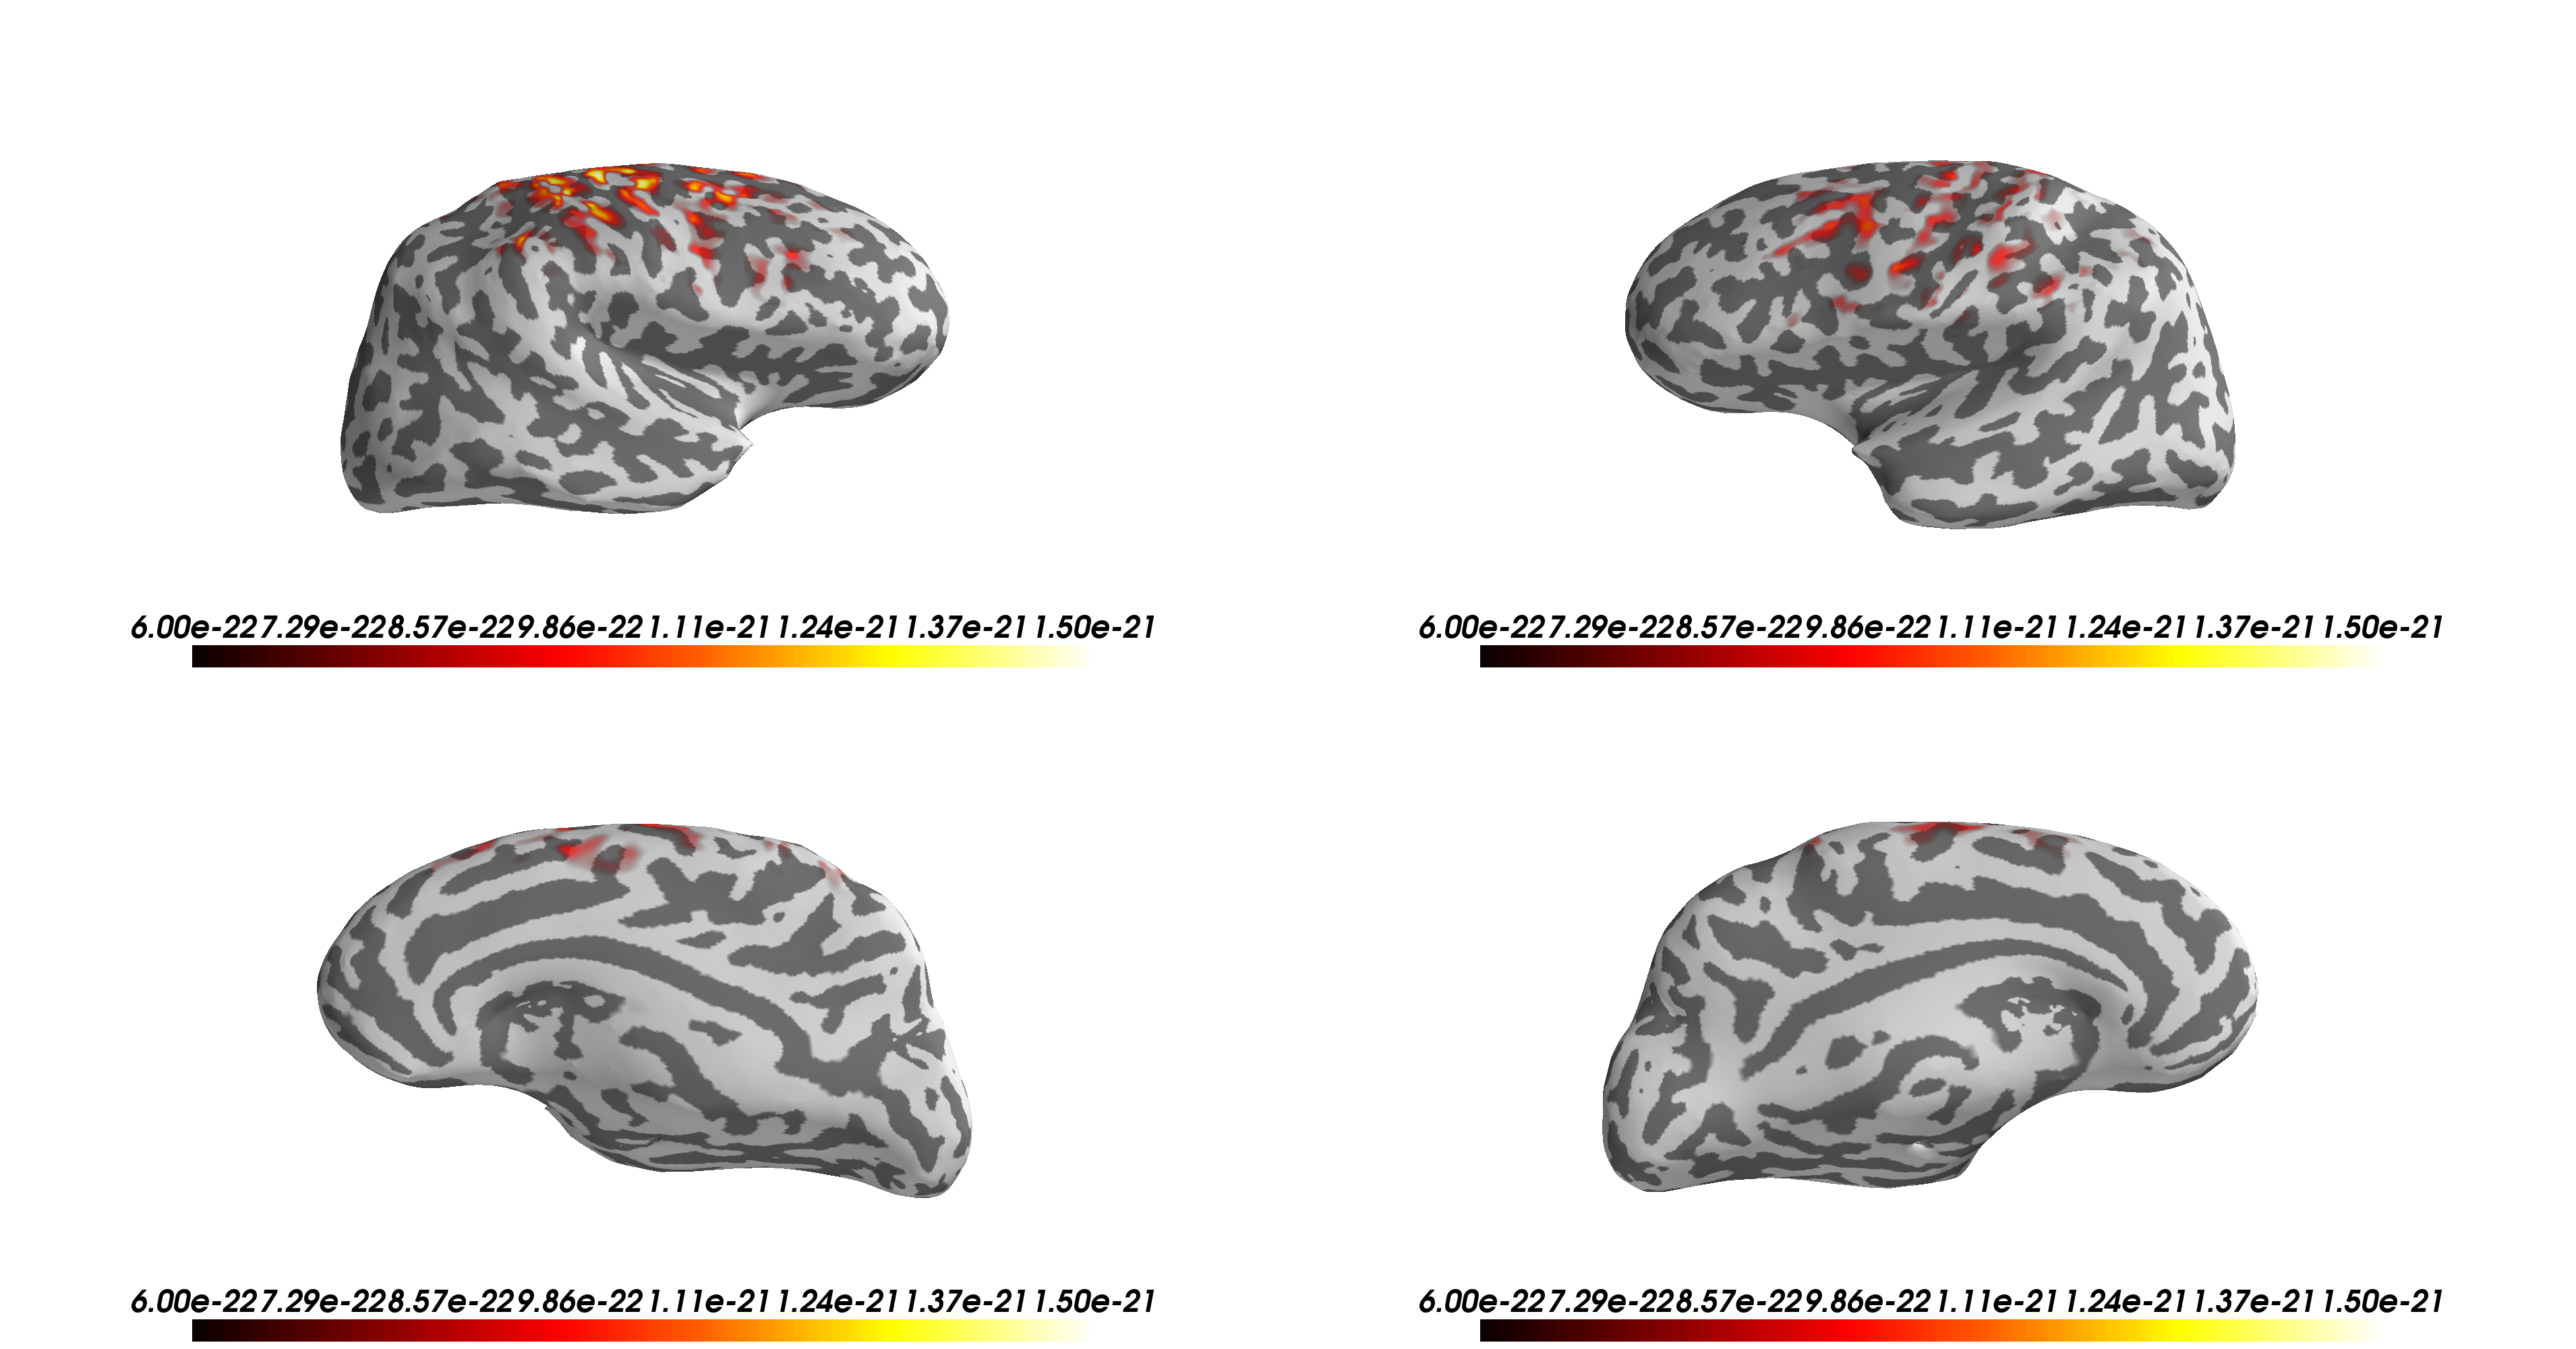
\includegraphics[width=\textwidth]{../images/psiicos_paper/Figure17_hr.jpg}
    \end{subfigure}
    \caption{Распределение индуцированной активности в бета-диапазоне (16--24 Гц)}\label{fig:beta_pwr}
\end{figure} %figure 17

\begin{figure}
    \begin{subfigure}[b]{0.5\textwidth}
        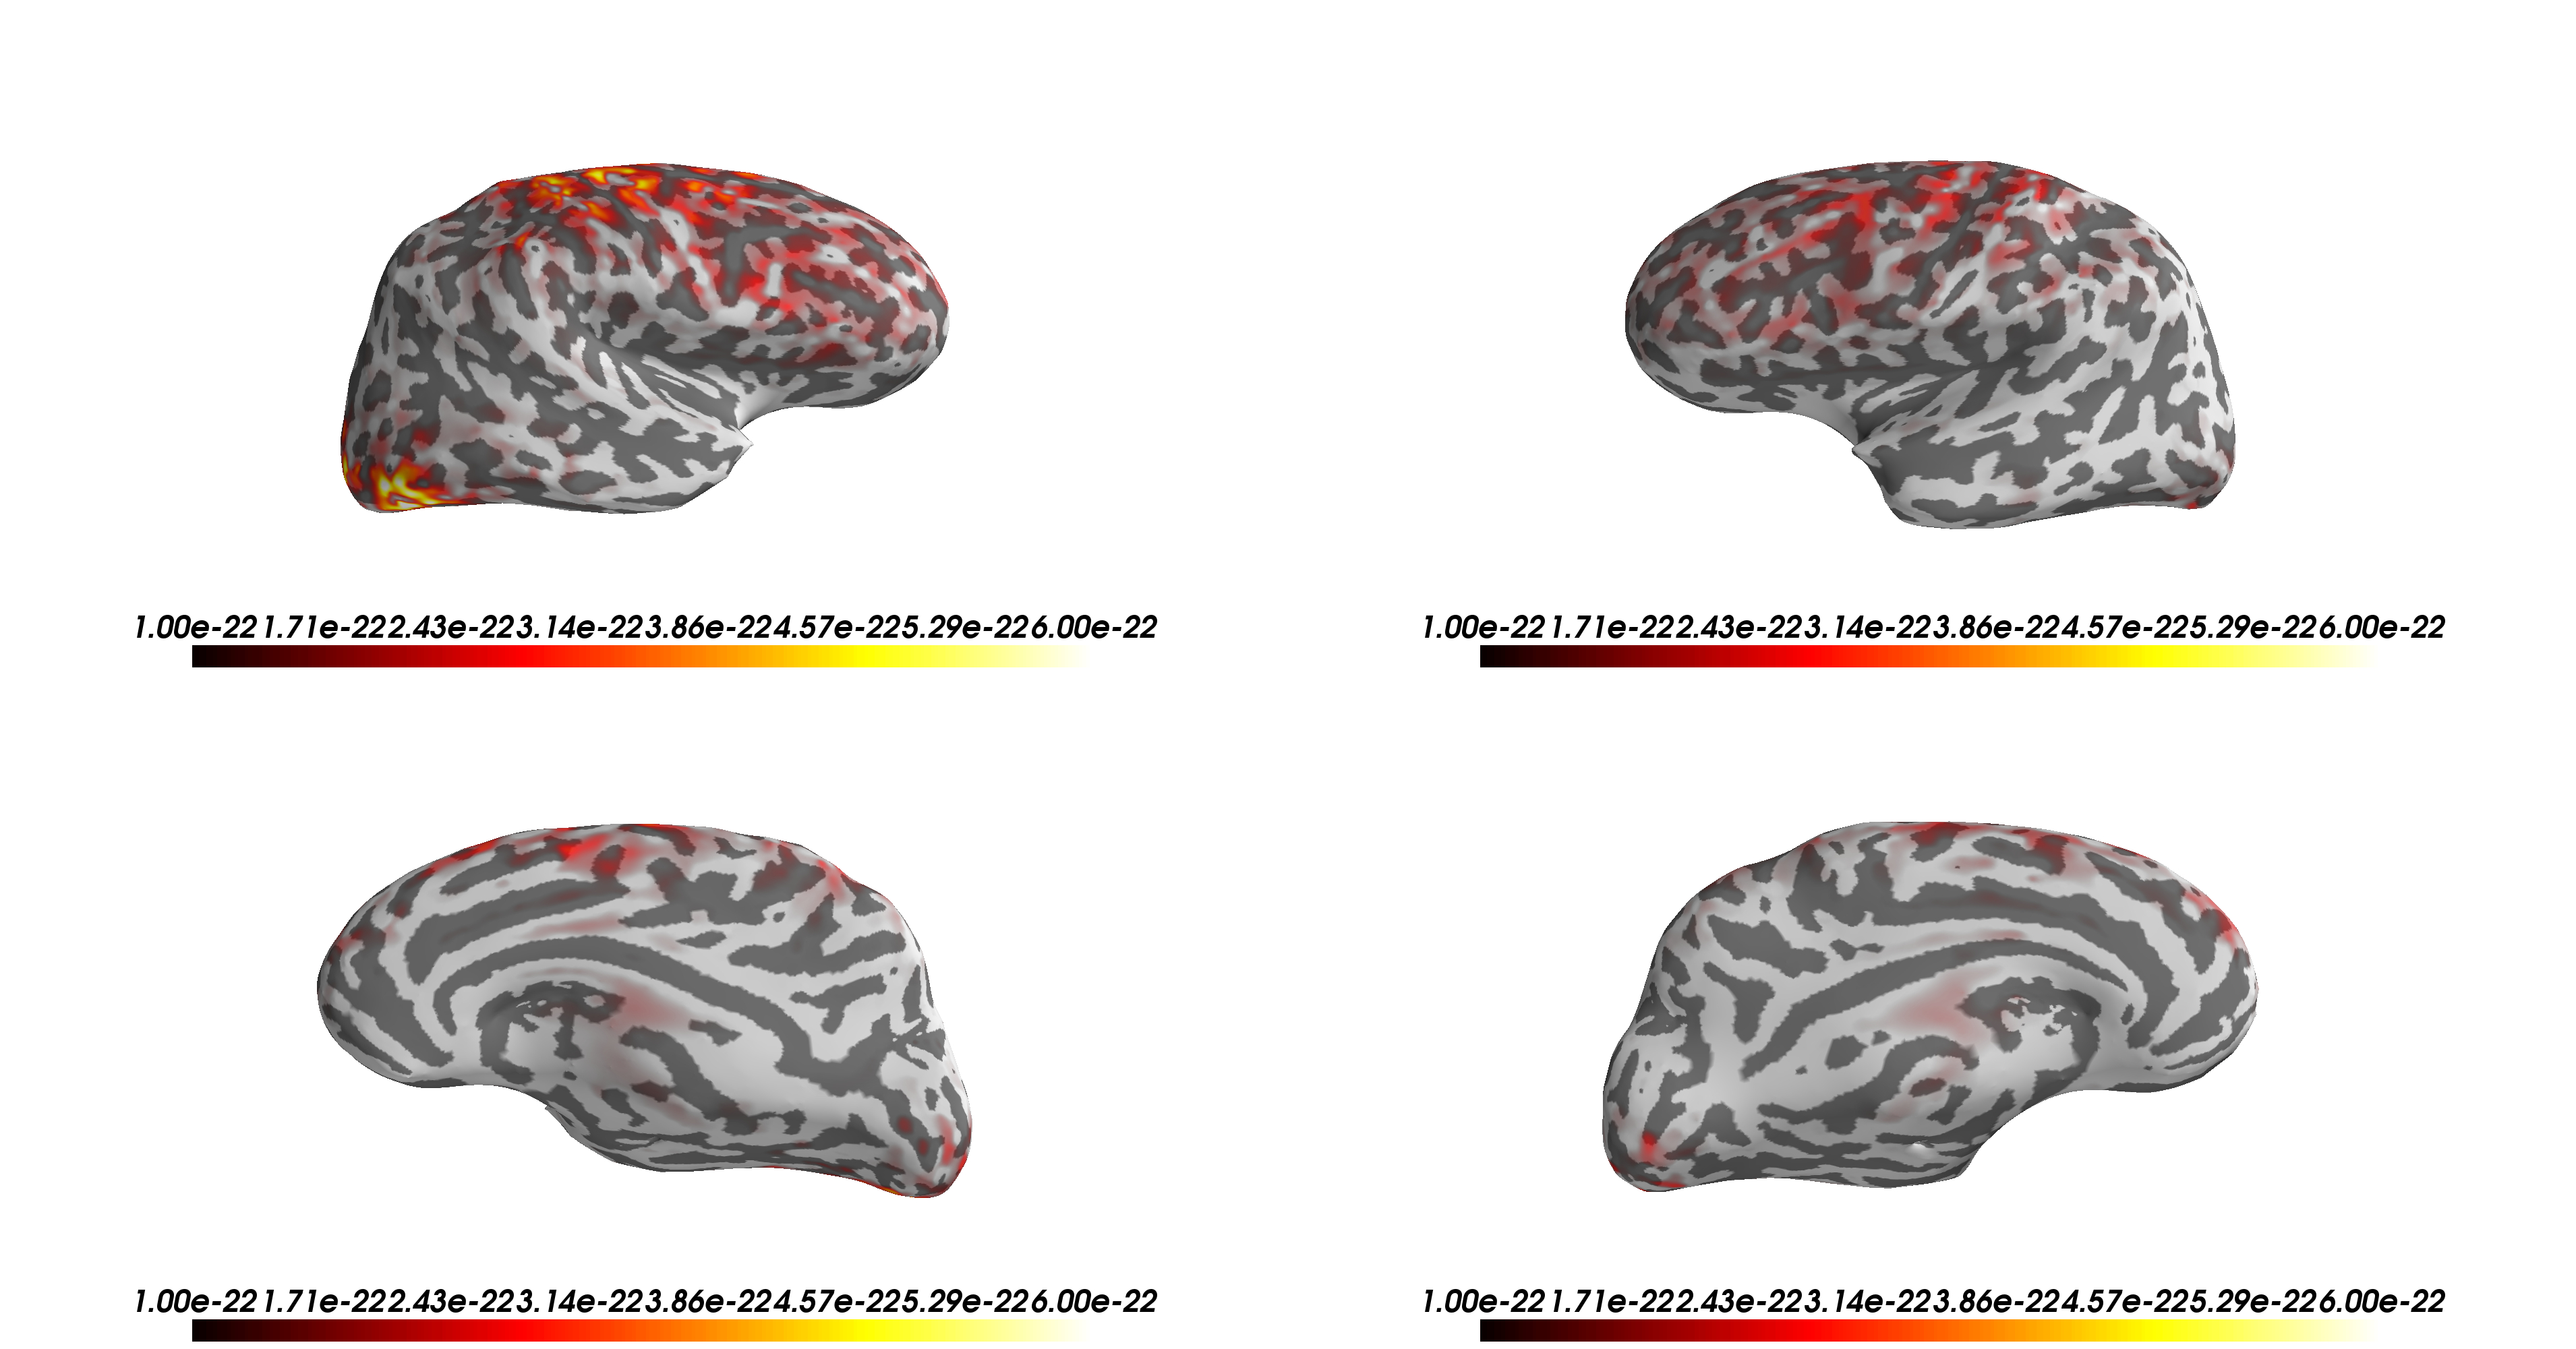
\includegraphics[width=\textwidth]{../images/psiicos_paper/Figure18a_hr.jpg}
        \caption{Нижний гамма-диапазон}\label{fig:lgama_pwr}
    \end{subfigure}
    % \vspace{1cm}
    \begin{subfigure}[b]{0.5\textwidth}
        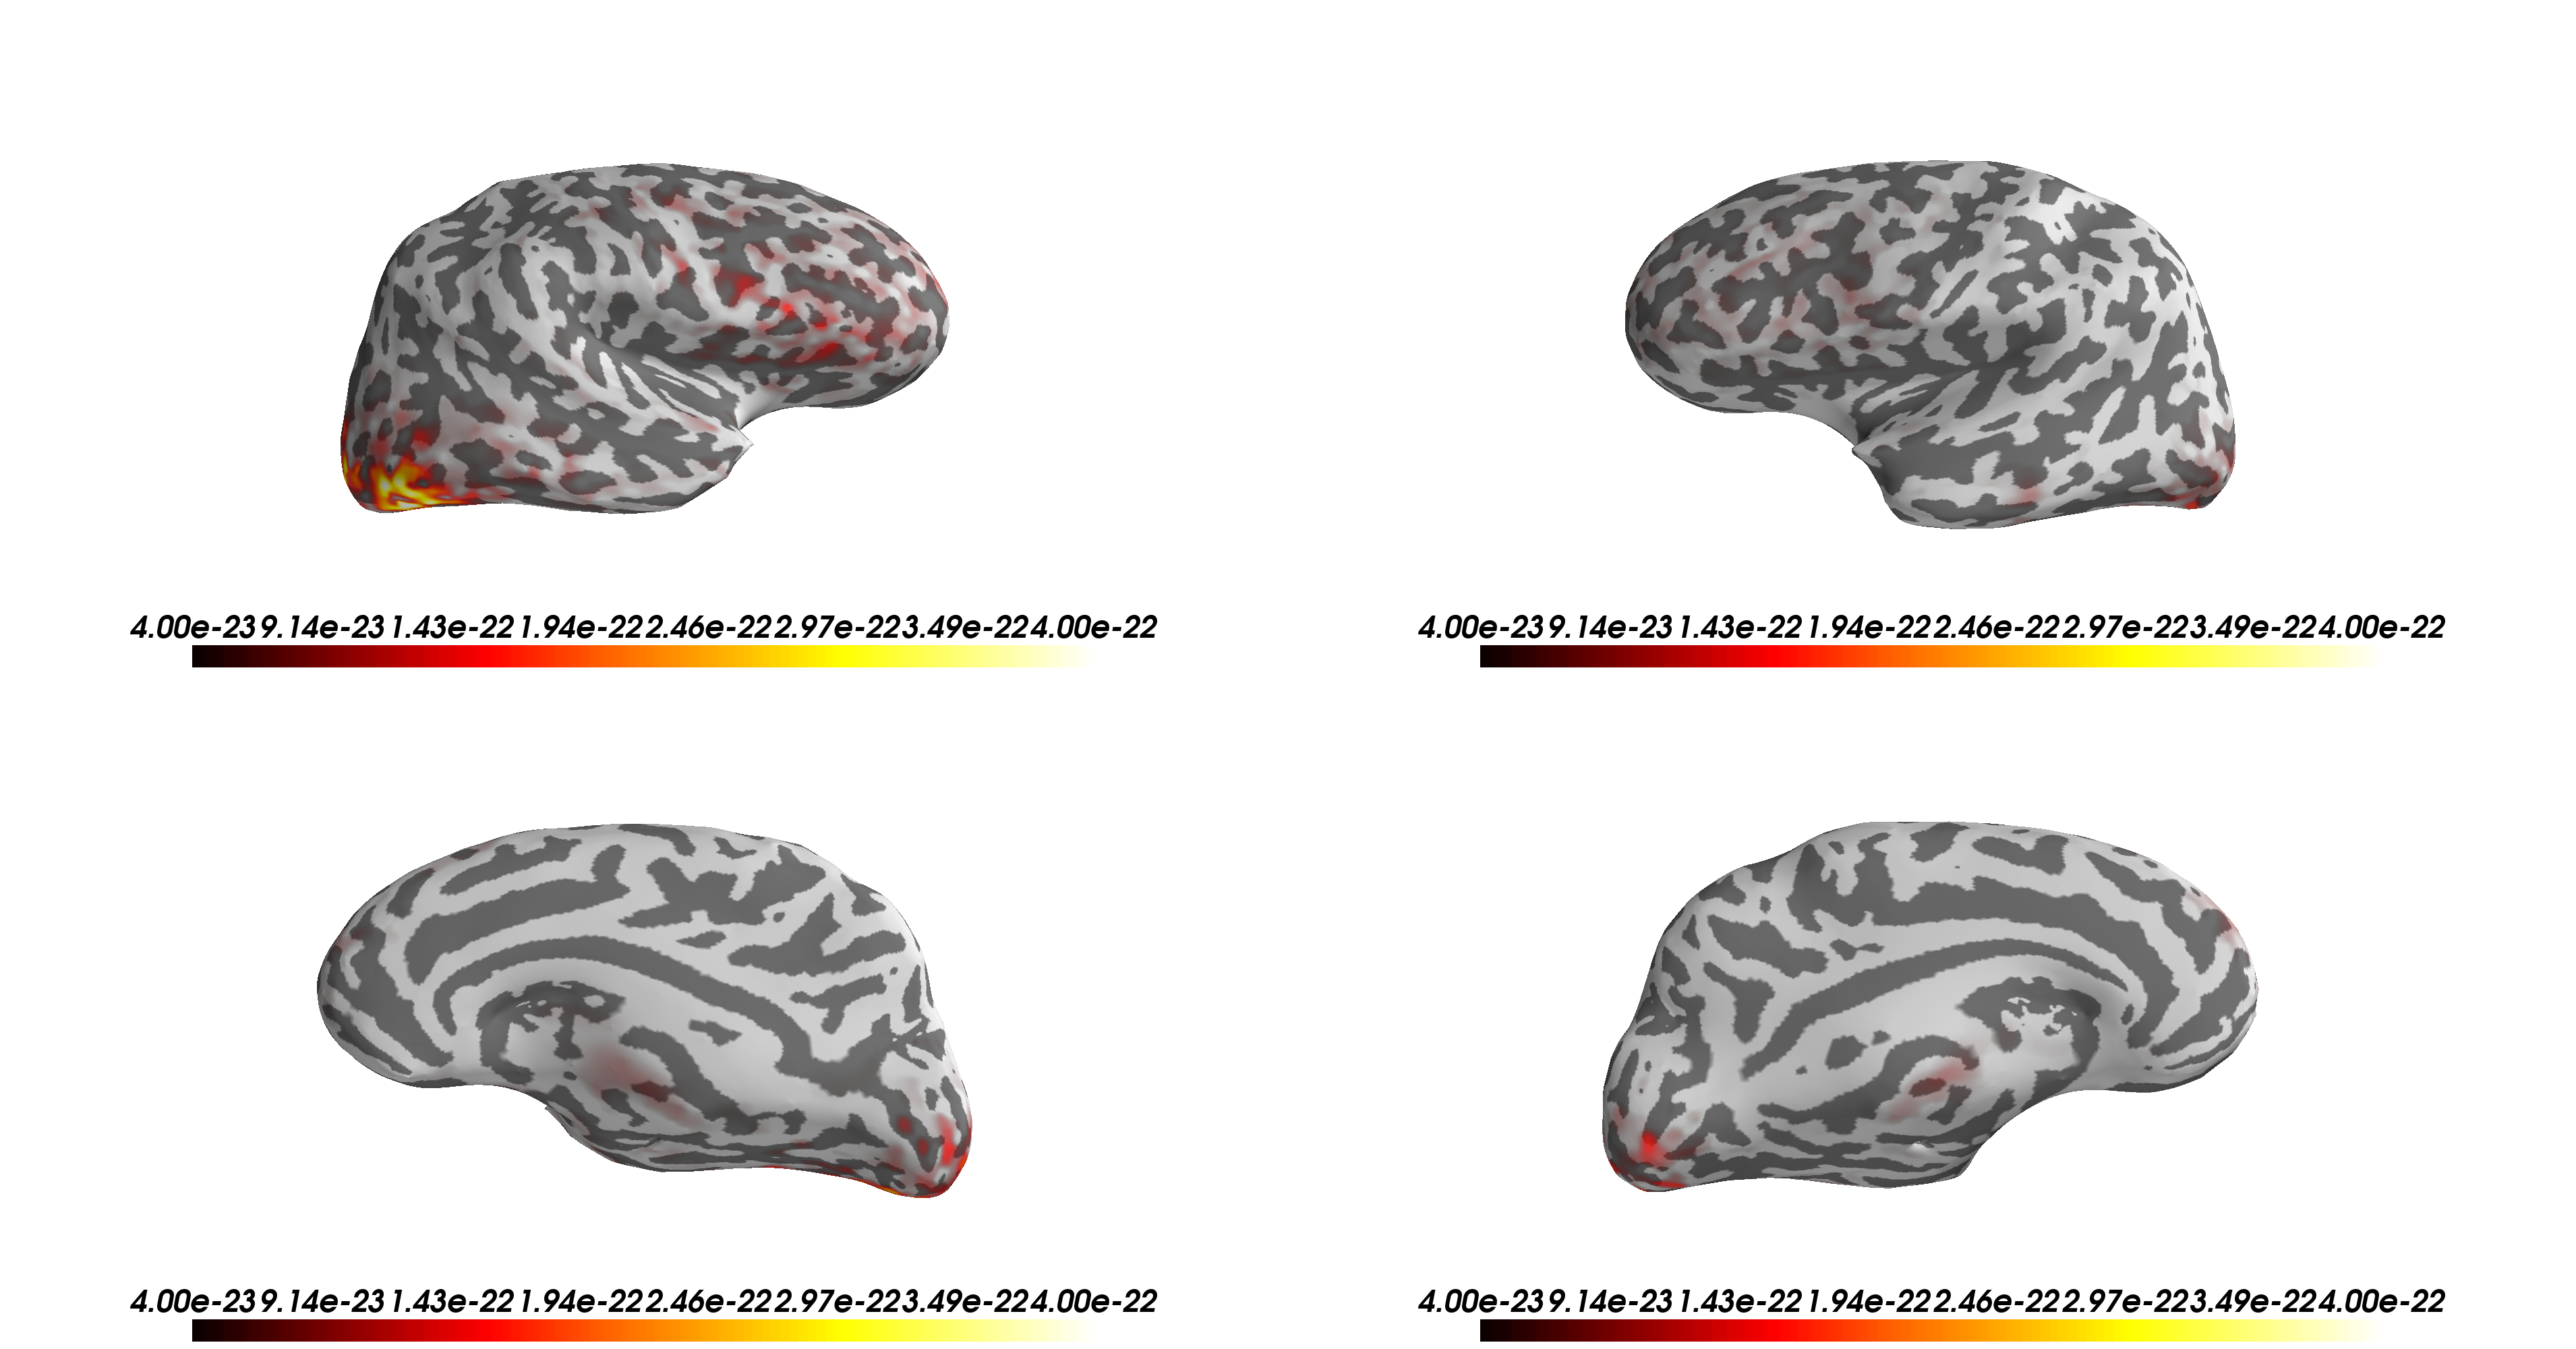
\includegraphics[width=0.99\textwidth]{../images/psiicos_paper/Figure18b_hr.jpg}
        \caption{Верхний гамма-диапазон}\label{fig:gama_pwr}
    \end{subfigure}
    \caption{Распределение индуцированной активности в нижнем (30--60 Гц) и верхнем (65--85 Гц) гамма-диапазонах.}\label{fig:gamma_pwr}
\end{figure} %figure 18
